\documentclass[11pt,a4paper]{article}
\usepackage[T2A]{fontenc}
\usepackage[utf8]{inputenc}
\usepackage[english,russian]{babel}
\usepackage[margin=19mm]{geometry}
\usepackage{amsmath,amssymb,graphicx,array,longtable,xurl}
\usepackage[hidelinks]{hyperref}
\usepackage{microtype}
\setlength{\parindent}{0pt}
\setlength{\parskip}{5pt}
\emergencystretch=3em
\title{Лабораторная работа 0\\Инфраструктура воспроизводимых экспериментов}
\author{Ван Чжаофу\\ТПУ, курс «Нейронные сети»}
\date{2026}
\begin{document}
\maketitle

Автор: Ван Чжаофу. Курс «Нейронные сети». Отчёт построен из сохранённых журналов; обозначения Rxx однозначно раскрываются в реестре RUN\_ID в конце документа.\par

Основание требований: lab0\_experiment\_harness\_1010.pdf, редакция 2.1 от 09.10.2026. Структура из шести разделов соответствует §28 исходного задания.\par

\section{Профиль и конфигурация}

Профиль \path{P3adf02}, хеш идентификатора \path{3adf0221499eacfc4e28050e33c8f0c4118d71ff1f3b161c5c9524754e2a36f9}. Исходный идентификатор не публикуется. Использованы CIFAR-10, доля train 0.25, ширина CNN 96, глубина 4, batch size 64, AdamW, начальная скорость 0.001, weight decay 0.0001, cosine schedule с одной эпохой прогрева. В окончательной программе K=12, CPU threads=2. Число параметров 252778 (R01).\par

Модель: 4 слоёв Conv2d 3\(\times\)3 со stride=1, padding=1 и bias, после каждого ReLU; после первых 3 свёрток MaxPool2d 2\(\times\)2. Все скрытые каналы равны 96. Затем global average pooling, flatten и Linear 96\(\to\)10. BatchNorm, dropout и аугментации отсутствуют.\par

Из официальных 50000 обучающих изображений выделены train=43000, val=5000, cal=2000; test=10000 сохраняется отдельно. Для ЛР0 используется 10750 изображений train. Разбиение стратифицировано, seed=1729; доля применяется только к train. Нормализация рассчитана только по train; cal и test не использовались для обучения или подбора. Учебный файл протокола отсутствует, поэтому нельзя утверждать совпадение индексов с файлом преподавателя. Хеш разбиения \path{1fb3cce79756298949821689d00533bb092604dd2d41a3d687de0fd02bf83574} (R01).\par

Окружение: Python 3.11.17, PyTorch 2.7.1+cu126, CUDA 12.6, cuDNN 90701. GPU: RTX 3060 Laptop 6 GB. Режим A: CPU/deterministic/без AMP/workers=0; B: CUDA/deterministic/без AMP; C: CUDA с AMP. Workers=2 отдельно обозначен как вмешательство режима C, хотя таблица §12.1 включает эти прогоны в общий CPU-бюджет.\par

Начальная попытка K=10 не прошла условие уменьшения loss вдвое: 1.9642590621\(\to\)0.9827822588, отношение 0.500332. RUN\_ID \path{187f3bd4a93cd598f53b-47b8eee4daa145949b8406914abff222} сохранён и не объявлен успешным. После проверки журналов выбрана проверяемая коррекция --- K=12 с полным переобучением; профиль и исходные данные не изменены. Это изменение длительности, а не продолжение старой cosine-траектории. Измеренная стоимость эпохи около 24 s, оценка 13\(\cdot\)12\(\cdot\)24\(\approx\)3744 s без дополнительных CUDA-проверок; фактическое время основного serial-suite (без ранее выполненного E0 и последующих дополнительных CF4/profiling) 65.05 min. Бюджетный RUN\_ID \path{e592bd6f1f2da6e9f959-f1f208b3b6844b71a89d774e5e291a44}. Бюджетные прогоны не считаются E0. Тестируемый commit основной серии \path{5abedb11663b56690456dca8e8fa3dba24fbb3a7}.\par

\section{Устройство harness}
\begin{align*}
\mathrm{EXP\_ID}&=\operatorname{SHA256}(C,\Theta,D,S)_{0:20},\\
\mathrm{RUN\_ID}&=\mathrm{EXP\_ID}\,\Vert\,\mathrm{UUID}.
\end{align*}

Семь стадий: resolved config \(\to\) данные и split \(\to\) модель \(\to\) optimizer/scheduler \(\to\) ExperimentRunner \(\to\) validation/evaluation \(\to\) артефакты. Общие модули используются всеми условиями. Параметры находятся в YAML, переопределения сохраняются в resolved config.\par

\begin{figure}[htbp]\centering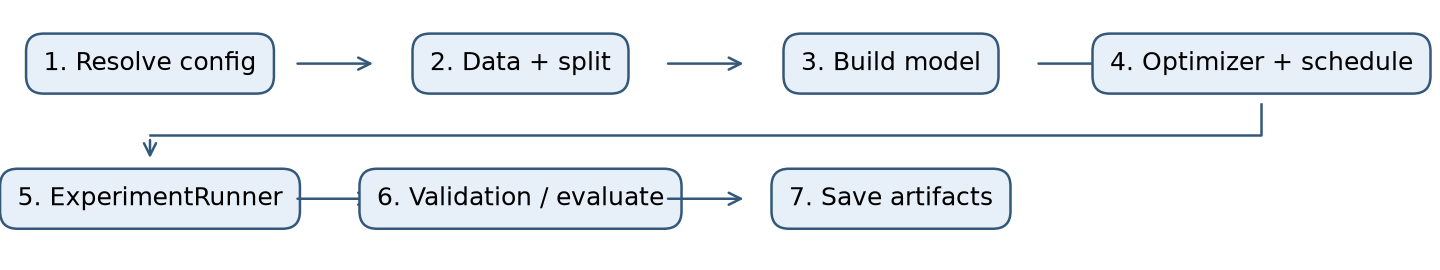
\includegraphics[width=\linewidth]{images/harness.png}\caption{Схема семи стадий harness}\end{figure}

EXP\_ID --- первые 20 шестнадцатеричных символов SHA256 канонического описания commit/dirty/source hash, resolved config, data/split fingerprint и seed. RUN\_ID дополняет EXP\_ID независимым UUID. Окружение отдельно записывается в manifest. Изменение результатов не меняет статус исходного кода: область проверки Git явно ограничена src/tests/scripts/configs/pyproject. Между парными прогонами код не коммитировался. Для грязных разработческих прогонов дополнительно сохраняется снимок исходников.\par

Manifest содержит оба ID, дату, профиль и student hash, Git commit/dirty/source hash, config/data/split hashes, режим, версии, lock hash, устройство, параметры и путь к resolved config. Малые текстовые результаты и split входят в Git; datasets/checkpoints/plots исключены. Без checkpoint теряются точное состояние оптимизатора и возможность немедленного продолжения; воспроизведение потребует повторного обучения.\par

Checkpoint содержит model, optimizer, scheduler, epoch, фактический global step, Python/NumPy/Torch/CUDA RNG, generator DataLoader, AMP GradScaler. Восстановление поддерживается на границе полной эпохи. Новый процесс создаёт новый RUN\_ID и указывает родительский RUN\_ID. При AMP пропущенное из-за overflow обновление не считается шагом оптимизатора. Неравные микробатчи при накоплении взвешиваются по числу объектов.\par

Логи хранят loss, accuracy, lr, epoch/step/time; отдельно сохраняется loss каждого mini-batch. Профилирование использует синхронизацию CUDA до и после интервала, не менее 50 прогревов и 100 измерений на batch size. Все числа ниже рассчитаны из этих файлов.\par

Проверка выпуска: 25 автоматических тестов; failures=0, errors=0, skipped=0, 20.400 s (tests-lab0-release.xml). Тесты обучения используют маркированные synthetic fixtures и не заменяют реальные эксперименты ниже.\par

\section{Результаты E0--E4}
\begin{align*}
\overline m&=\frac1N\sum_{i=1}^{N}m_i,&
s_m&=\sqrt{\frac{\sum_i(m_i-\overline m)^2}{N-1}},\\
\mathrm{CI}_{95\%}&=\overline m\pm t_{0.975,N-1}\frac{s_m}{\sqrt N},&
\Delta_\theta&=\frac{\lVert\theta_A-\theta_B\rVert_2}{\lVert\theta_A\rVert_2+10^{-12}}.
\end{align*}

\begin{figure}[htbp]\centering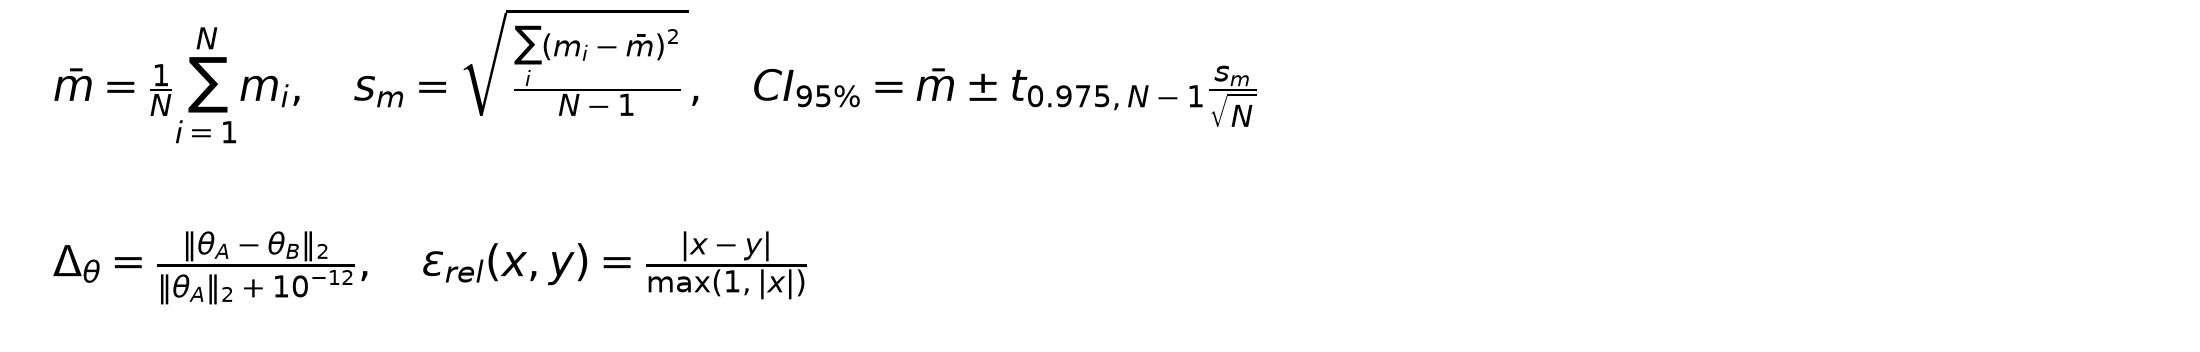
\includegraphics[width=\linewidth]{images/metric_definitions.png}\caption{Определения статистик и относительных расхождений}\end{figure}

E0 (R01): train loss 1.964259\(\to\)0.895176; отношение 0.455732; validation accuracy 0.6232. Независимый evaluate воспроизвёл итоговую accuracy. Условия приёмки: PASS.\par

\begin{figure}[htbp]\centering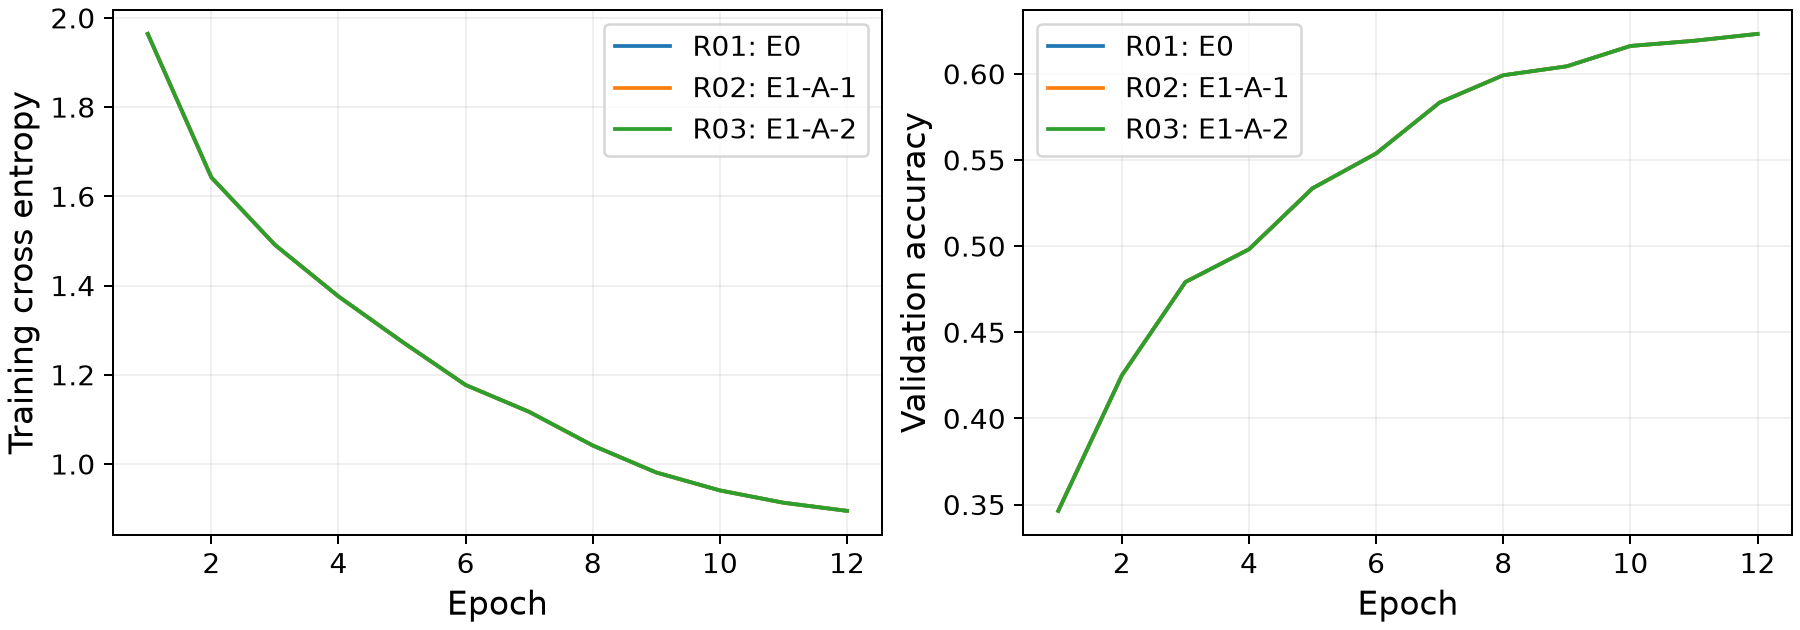
\includegraphics[width=\linewidth]{images/learning_curves.png}\caption{Кривые обучения}\end{figure}


E1 и E3:\par

\begingroup\scriptsize\setlength{\tabcolsep}{2pt}
\begin{longtable}{|>{\raggedright\arraybackslash}p{\dimexpr\linewidth/8-2\tabcolsep-2\arrayrulewidth\relax}|>{\raggedright\arraybackslash}p{\dimexpr\linewidth/8-2\tabcolsep-2\arrayrulewidth\relax}|>{\raggedright\arraybackslash}p{\dimexpr\linewidth/8-2\tabcolsep-2\arrayrulewidth\relax}|>{\raggedright\arraybackslash}p{\dimexpr\linewidth/8-2\tabcolsep-2\arrayrulewidth\relax}|>{\raggedright\arraybackslash}p{\dimexpr\linewidth/8-2\tabcolsep-2\arrayrulewidth\relax}|>{\raggedright\arraybackslash}p{\dimexpr\linewidth/8-2\tabcolsep-2\arrayrulewidth\relax}|>{\raggedright\arraybackslash}p{\dimexpr\linewidth/8-2\tabcolsep-2\arrayrulewidth\relax}|>{\raggedright\arraybackslash}p{\dimexpr\linewidth/8-2\tabcolsep-2\arrayrulewidth\relax}|}\hline
Режим & E1 runs & max \(\varepsilon\)rel(loss) & \(\Delta\)accuracy & E1 & E3 runs & \(\Delta\)\(\theta\) & E3 \\\hline
\endhead
A & R02/R03 & 0 & 0 & PASS & R04/R06 & 0 & PASS \\\hline
B & R07/R08 & 0 & 0 & PASS & R09/R11 & 0 & PASS \\\hline
C & R12/R13 & 0 & 0 & PASS & R14/R16 & 0 & PASS \\\hline
\end{longtable}\endgroup

В A требуются точные траектории и метрика, \(\Delta\)\(\theta\)\(\leq\)1e-7; в B --- \(\varepsilon\)rel(loss)\(\leq\)1e-5, \(\Delta\)accuracy\(\leq\).001 и \(\Delta\)\(\theta\)\(\leq\)1e-5. В C численные пороги не заданы: таблица сообщает измерение, а не универсальную гарантию. Во всех режимах проверены split, first-batch checksum и число реальных обновлений. A: continuous/resume=2016/2016, пропущено из-за overflow=0; B: continuous/resume=2016/2016, пропущено из-за overflow=0; C: continuous/resume=2015/2015, пропущено из-за overflow=1.\par

\begin{figure}[htbp]\centering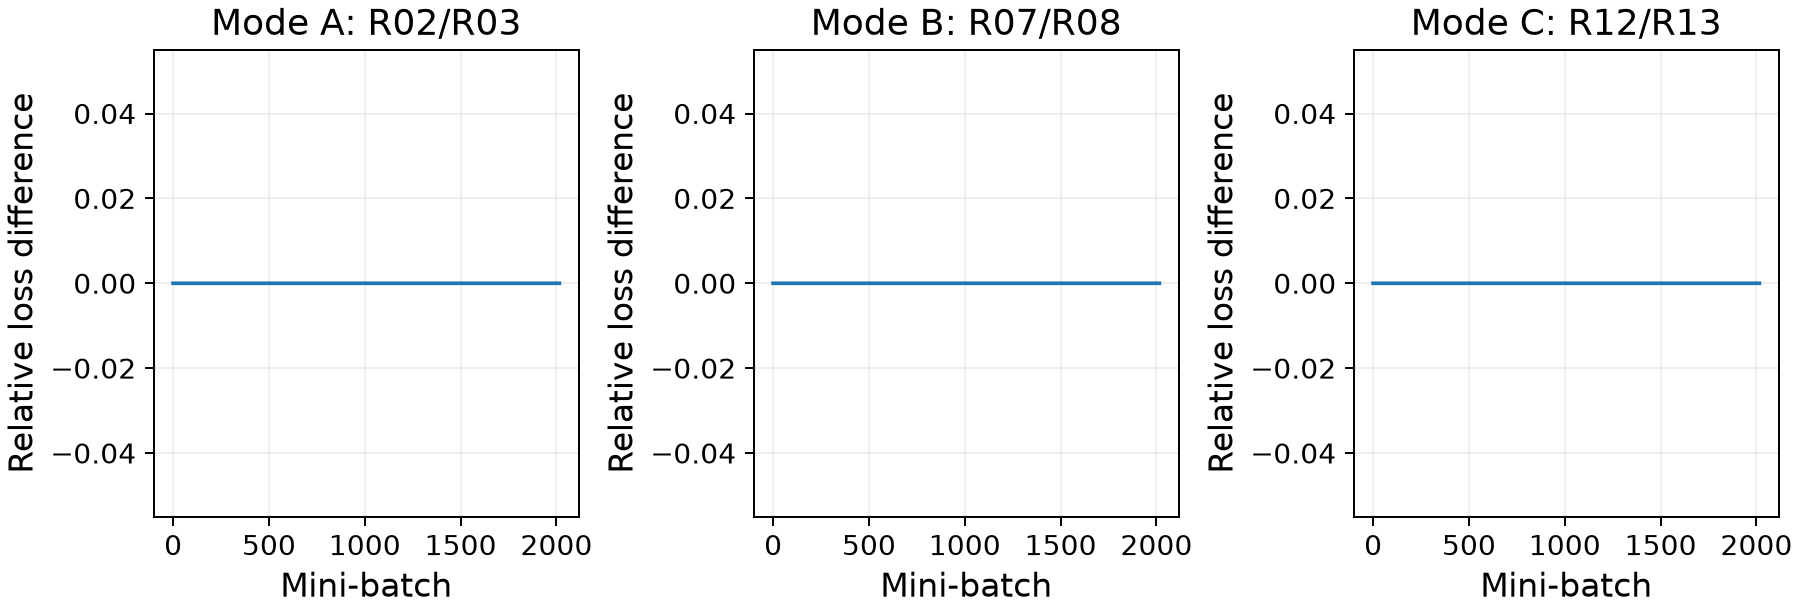
\includegraphics[width=\linewidth]{images/repeatability.png}\caption{Разности траекторий}\end{figure}

\begin{figure}[htbp]\centering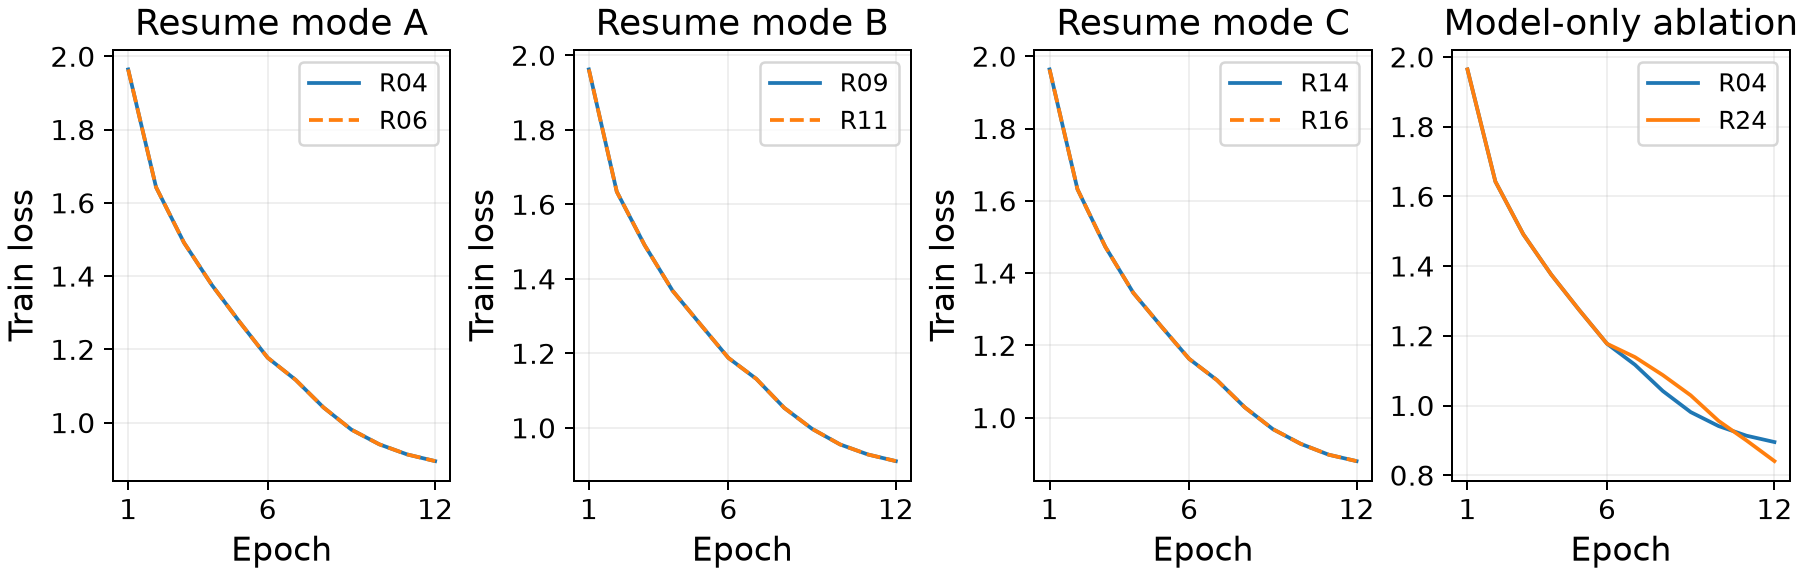
\includegraphics[width=\linewidth]{images/resume_and_ablation.png}\caption{Полное восстановление и усечение checkpoint}\end{figure}

E2 (R17, R18, R19, R20, R21): N=5, средняя validation accuracy=0.633440, выборочное стандартное отклонение=0.008708, 95\% Student t CI=[0.622628; 0.644252]. Все пять seeds различны; split и остальные условия фиксированы. Ориентир PDF для минимального эффекта --- 2s=0.017416. Разброс не превышает 1.5 п.п.\par

\begin{figure}[htbp]\centering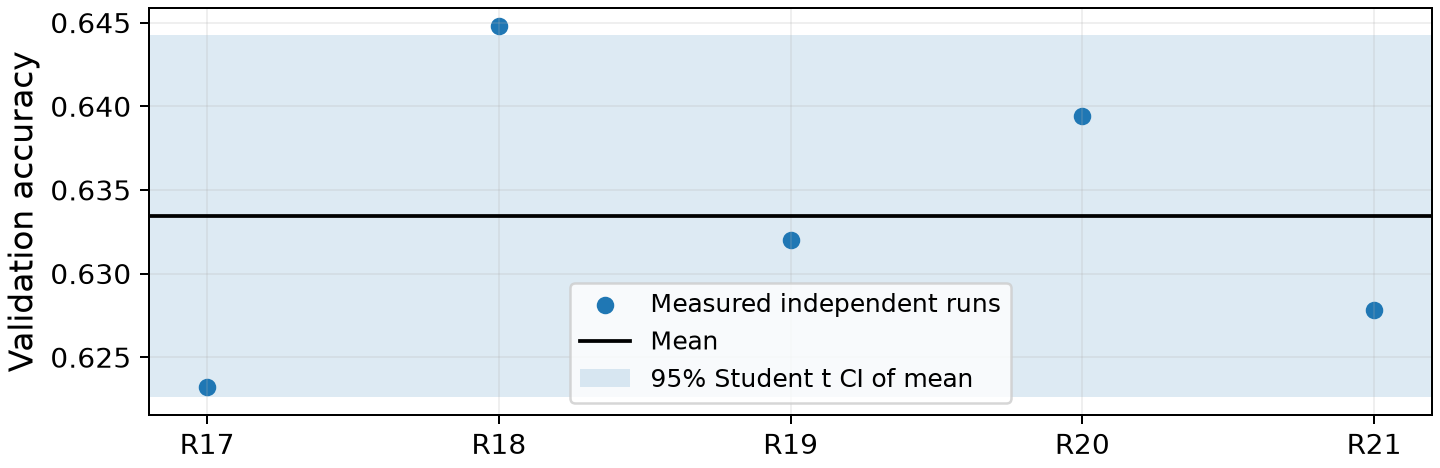
\includegraphics[width=\linewidth]{images/seed_variance.png}\caption{Разброс по seeds}\end{figure}

E4: источник обученных весов --- R02; raw samples находятся в E4-cpu-registered.json/E4-cuda-registered.json серии; исходные замеры E4-cpu.json/E4-cuda.json также сохранены. Forward-only latency отличается от времени training step; длительность эпох берётся из training logs, а не выводится из forward throughput.\par


Отдельный E4 RUN\_ID для cpu: \path{c29fec693e78f31bd03b-2afa25ee666d4ce4823bf95d43f5c1a8}; источник весов \path{6a750eb4531ac754cde7-b798991a1a7b457cbb0de2144b2a4742}. Измерений на B: 100; прогревов не менее 50. Входы --- явно заданные тензоры нормального распределения формы B\(\times\)3\(\times\)32\(\times\)32; это замеры времени, не оценка accuracy.\par

\subsection*{E4, cpu}

\begingroup\scriptsize\setlength{\tabcolsep}{2pt}
\begin{longtable}{|>{\raggedright\arraybackslash}p{\dimexpr\linewidth/7-2\tabcolsep-2\arrayrulewidth\relax}|>{\raggedright\arraybackslash}p{\dimexpr\linewidth/7-2\tabcolsep-2\arrayrulewidth\relax}|>{\raggedright\arraybackslash}p{\dimexpr\linewidth/7-2\tabcolsep-2\arrayrulewidth\relax}|>{\raggedright\arraybackslash}p{\dimexpr\linewidth/7-2\tabcolsep-2\arrayrulewidth\relax}|>{\raggedright\arraybackslash}p{\dimexpr\linewidth/7-2\tabcolsep-2\arrayrulewidth\relax}|>{\raggedright\arraybackslash}p{\dimexpr\linewidth/7-2\tabcolsep-2\arrayrulewidth\relax}|>{\raggedright\arraybackslash}p{\dimexpr\linewidth/7-2\tabcolsep-2\arrayrulewidth\relax}|}\hline
B & mean ms & median ms & p95 ms & samples/s & CV & peak GPU MiB \\\hline
\endhead
1 & 1.1572 & 1.1524 & 1.1914 & 864.12 & 0.0163 & n/a \\\hline
16 & 13.6443 & 13.5893 & 14.2845 & 1172.65 & 0.0219 & n/a \\\hline
64 & 53.6907 & 53.5572 & 54.7072 & 1192.01 & 0.0101 & n/a \\\hline
256 & 215.7320 & 214.8388 & 219.6980 & 1186.66 & 0.0158 & n/a \\\hline
\end{longtable}\endgroup


CV>10\% при B=[]. Число повторов увеличено по сравнению с исходными 30 до 100; все замеры сохранены. Порог CV соблюдён для всех B.\par


Отдельный E4 RUN\_ID для cuda: \path{724bae602e86195355ad-dbf545e3a7da421e9daf3626733fb95d}; источник весов \path{6a750eb4531ac754cde7-b798991a1a7b457cbb0de2144b2a4742}. Измерений на B: 100; прогревов не менее 50. Входы --- явно заданные тензоры нормального распределения формы B\(\times\)3\(\times\)32\(\times\)32; это замеры времени, не оценка accuracy.\par

\subsection*{E4, cuda}

\begingroup\scriptsize\setlength{\tabcolsep}{2pt}
\begin{longtable}{|>{\raggedright\arraybackslash}p{\dimexpr\linewidth/7-2\tabcolsep-2\arrayrulewidth\relax}|>{\raggedright\arraybackslash}p{\dimexpr\linewidth/7-2\tabcolsep-2\arrayrulewidth\relax}|>{\raggedright\arraybackslash}p{\dimexpr\linewidth/7-2\tabcolsep-2\arrayrulewidth\relax}|>{\raggedright\arraybackslash}p{\dimexpr\linewidth/7-2\tabcolsep-2\arrayrulewidth\relax}|>{\raggedright\arraybackslash}p{\dimexpr\linewidth/7-2\tabcolsep-2\arrayrulewidth\relax}|>{\raggedright\arraybackslash}p{\dimexpr\linewidth/7-2\tabcolsep-2\arrayrulewidth\relax}|>{\raggedright\arraybackslash}p{\dimexpr\linewidth/7-2\tabcolsep-2\arrayrulewidth\relax}|}\hline
B & mean ms & median ms & p95 ms & samples/s & CV & peak GPU MiB \\\hline
\endhead
1 & 0.6578 & 0.6619 & 0.6797 & 1520.19 & 0.0236 & 34.04 \\\hline
16 & 1.2995 & 1.2944 & 1.3372 & 12312.81 & 0.0191 & 45.15 \\\hline
64 & 1.5343 & 1.5352 & 1.5776 & 41711.69 & 0.0381 & 81.72 \\\hline
256 & 5.1167 & 5.1001 & 5.1928 & 50032.69 & 0.0173 & 227.97 \\\hline
\end{longtable}\endgroup


CV>10\% при B=[]. Число повторов увеличено по сравнению с исходными 30 до 100; все замеры сохранены. Порог CV соблюдён для всех B.\par


Время полной эпохи (обучение и validation), фактические журналы E1:\par

\begingroup\scriptsize\setlength{\tabcolsep}{2pt}
\begin{longtable}{|>{\raggedright\arraybackslash}p{\dimexpr\linewidth/4-2\tabcolsep-2\arrayrulewidth\relax}|>{\raggedright\arraybackslash}p{\dimexpr\linewidth/4-2\tabcolsep-2\arrayrulewidth\relax}|>{\raggedright\arraybackslash}p{\dimexpr\linewidth/4-2\tabcolsep-2\arrayrulewidth\relax}|>{\raggedright\arraybackslash}p{\dimexpr\linewidth/4-2\tabcolsep-2\arrayrulewidth\relax}|}\hline
Режим / run & mean epoch s & p95 epoch s & peak training GPU MiB \\\hline
\endhead
A / R02 & 23.453 & 24.392 & 0.00 \\\hline
B / R07 & 2.227 & 2.366 & 150.87 \\\hline
C / R12 & 2.521 & 2.764 & 116.38 \\\hline
\end{longtable}\endgroup

Дополнительная проверка устойчивости GPU timing: RUN\_ID \path{efe887782e2794dfe859-e0ce03d1443a4128b6f5749b42fcc1fb}, измеренный прогрев не менее секунды на каждом B, затем 50 дополнительных warmup и 300 измерений. Она не заменяет предписанную серию выше; все три серии сохранены.\par

\begingroup\scriptsize\setlength{\tabcolsep}{2pt}
\begin{longtable}{|>{\raggedright\arraybackslash}p{\dimexpr\linewidth/6-2\tabcolsep-2\arrayrulewidth\relax}|>{\raggedright\arraybackslash}p{\dimexpr\linewidth/6-2\tabcolsep-2\arrayrulewidth\relax}|>{\raggedright\arraybackslash}p{\dimexpr\linewidth/6-2\tabcolsep-2\arrayrulewidth\relax}|>{\raggedright\arraybackslash}p{\dimexpr\linewidth/6-2\tabcolsep-2\arrayrulewidth\relax}|>{\raggedright\arraybackslash}p{\dimexpr\linewidth/6-2\tabcolsep-2\arrayrulewidth\relax}|>{\raggedright\arraybackslash}p{\dimexpr\linewidth/6-2\tabcolsep-2\arrayrulewidth\relax}|}\hline
B & initial mean ms / N100 & registered mean ms / N100 & extra mean ms / N300 & extra CV & SM MHz before\(\to\)after \\\hline
\endhead
1 & 0.6639 & 0.6578 & 0.6559 & 0.2081 & 1425\(\to\)1425 \\\hline
16 & 0.6810 & 1.2995 & 1.2208 & 0.1362 & 1425\(\to\)1620 \\\hline
64 & 1.4781 & 1.5343 & 1.4594 & 0.0301 & 1620\(\to\)1710 \\\hline
256 & 5.1531 & 5.1167 & 5.1799 & 0.0239 & 1717\(\to\)1575 \\\hline
\end{longtable}\endgroup

В дополнительной серии порог CV не достигнут при B=[1, 16]. Увеличение N до 300 и дополнительный прогрев не устранили вариативность. Для B16 наблюдалось изменение частоты SM, но по этим данным нельзя приписать все выбросы частоте или полностью разделить GPU clock variation и задержки запуска на host. Поэтому устойчивость latency вне конкретной серии не установлена; цифры для малых B имеют это ограничение. Сырые выбросы не исключались.\par

\begin{figure}[htbp]\centering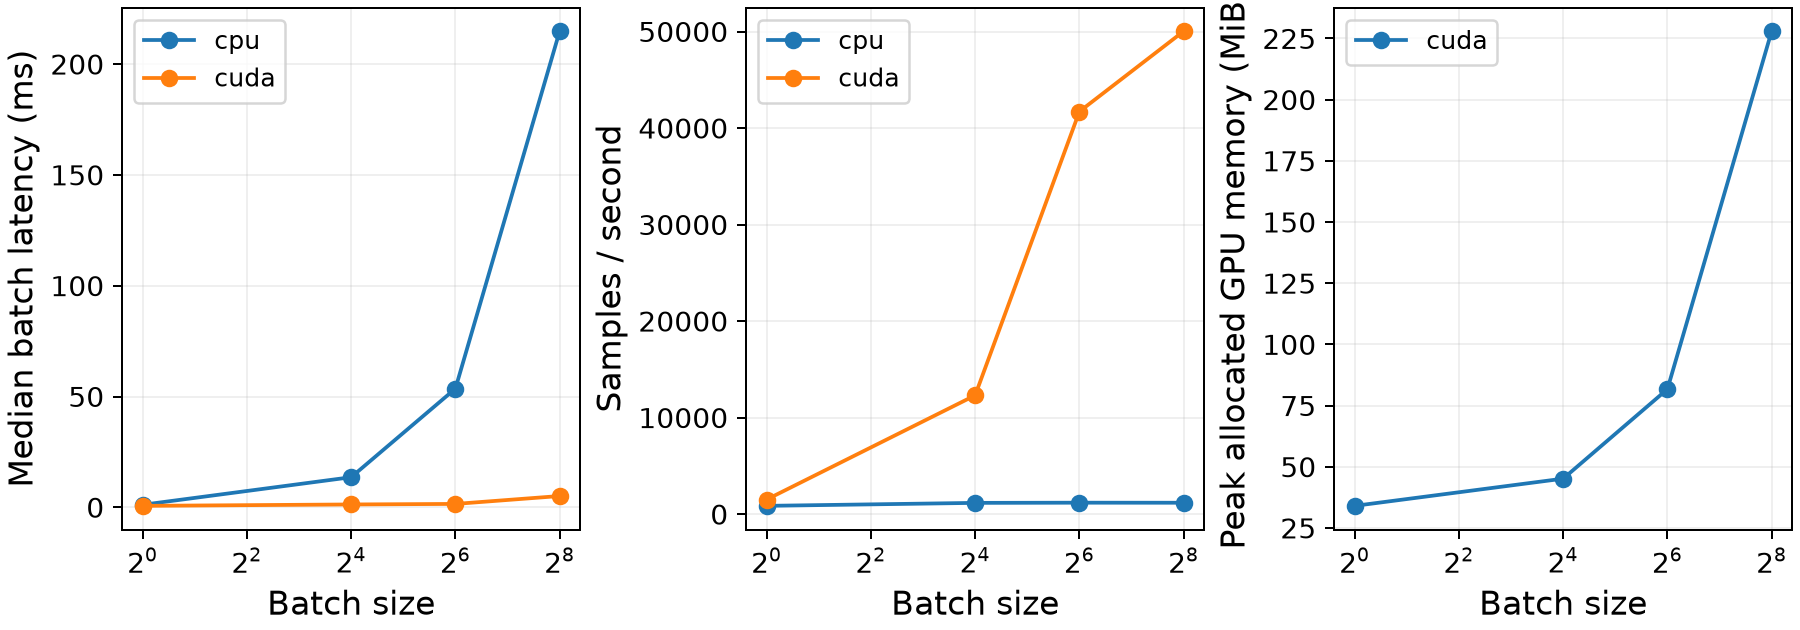
\includegraphics[width=\linewidth]{images/performance.png}\caption{Ресурсные характеристики}\end{figure}

\section{Уровни воспроизводимости}


Для режима A измеренная серия подтверждает R3 (наблюдаемое совпадение серии) в зафиксированном окружении. \par


Для режима B измеренная серия подтверждает R3 (наблюдаемое совпадение серии) в зафиксированном окружении. \par


Для режима C измеренная серия подтверждает R3 (наблюдаемое совпадение серии) в зафиксированном окружении. В C наблюдаемое совпадение объясняется фиксированными seed, потоком данных, алгоритмами и одним устройством; AMP сам по себе не вводит случайность. Это не обещание побитовой повторяемости для любых AMP/worker условий.\par


\section{Контрфактические вопросы}

1. По E2 среднее=0.633440, s=0.008708, ориентир 2s=0.017416 (R17, R18, R19, R20, R21). Это эвристика PDF, не рассчитанная мощность теста. При допущении независимых одинаково распределённых прогонов стандартная ошибка среднего убывает как N\textasciicircum{}(-1/2), поэтому для вдвое меньшего эффекта при фиксированных квантилях требуется примерно 4N=20 прогонов. Дополнительные 15 запусков означают около 72 min сверх принятой оценки всей серии около 62 min; без пересмотра исходного бюджета это не укладывается. При \textasciitilde{}24s/epoch и K=12 это около 96 min только на одну серию, без CUDA и диагностики. Точное число для заданной мощности требует заранее выбранного теста/альтернативы; из пяти измерений универсальную гарантию получить нельзя.\par

2. Два запуска workers=2: R22/R23; max \(\varepsilon\)rel(loss)=0, \(\Delta\)accuracy=0. При сопоставлении с workers=0 (R02) split, checksum первого batch и все 2016 step losses совпали; \(\Delta\)accuracy=0. В текущем pipeline отсутствуют случайные аугментации, порядок задаётся отдельным generator, workers получают фиксированные seed. Число workers изменяет выполнение загрузки, но в измеренной серии не изменило входные данные и арифметику модели; это объясняет отсутствие расхождения. Наблюдение не распространяется на произвольные аугментации и другие pipelines.\par

3. Усечённый checkpoint содержит только model.state\_dict; итог R24 против R04: \(\Delta\)\(\theta\)=0.37102801. Для локализации выполнен отдельный опыт RUN\_ID \path{699083a5d60b457b7a27-4565dcc8697040c498b47d8fedaae4d4}: одна и та же сохранённая точка и один и тот же градиент (loss=1.2374443). Сброс только моментов AdamW при прежней lr дал \(\Delta\)\(\theta\)=0.00982349; изменение только lr с 0.00057115742 на 0.001 при сохранённых моментах дало \(\Delta\)\(\theta\)=0.0015197029. Без generator state порядок следующего batch меняется: да. Loss контрольного batch совпал с реально записанным первым шагом эпохи 7. Таким образом, потеря моментов, положения schedule и порядка данных даёт независимо проверяемые источники расхождения. Локальные одношаговые разности нельзя складывать как разложение конечного \(\Delta\)\(\theta\). Для данного CNN нет dropout и случайных аугментаций; Python/NumPy/global Torch RNG сохранены для общего интерфейса, их отдельное влияние здесь не измерялось.\par

4. В исходной E2 из пяти seeds пары с |\(\Delta\)accuracy|<.001 не оказалось. Число дополнительных запусков по тому же протоколу: 3; дополнительный бюджет был заранее ограничен. Проверенные пары: R25/R27: accuracy=0.6364/0.6364, |\(\Delta\)accuracy|=0.000000, совпадение всех step losses --- нет, max \(\varepsilon\)rel(loss)=0.510981, различных step losses=2016. Основные mean/s/CI выше по-прежнему рассчитаны только по исходным пяти seeds. Близкая конечная accuracy не доказывает воспроизведение траектории; дополнительный поиск пары не является оценкой эффекта нового метода.\par

5. В manifest R02 сохранён cuDNN=90701. При замене версии изменится environment.cudnn, но не каноническая функция EXP\_ID, если код/config/data/seed прежние. Фактическая замена библиотеки не выполнялась. Происхождение R0 остаётся описываемым, R1 для сохранённого split можно проверить; R2/R3 после изменения окружения без повторных измерений не гарантируются.\par

6. Выполнены два состояния отдельной sandbox-копии data\_batch\_1 по одному и тому же имени и пути, размер не изменился. Диагностические RUN\_ID \path{86c8dd0011a17e664ca2-d4864d8b3e2446ebbd586261f081c1b9} и \path{26fbdb25ae58f6ba17cc-acc3b6459ddd475885825852351b1aa8}. SHA256 до изменения=54636561a3ce25bd3e19253c6b0d8538147b0ae398331ac4a2d86c6d987368cd, после изменения одного байта=8b0686ccaea34977c1f2443df1f75e662d8dd988fc1137c8050051f687b987e7. Изменились data fingerprint и EXP\_ID; config hash, split fingerprint, seed, Git commit, source hash и профиль остались прежними. У независимых диагностических запусков различаются RUN\_ID. Официальные обучающие файлы не изменялись. MD5-проверка CIFAR дополнительно отклонила бы испорченный файл до обучения.\par

7. Для B=1 CPU first forward=3.3674 ms, median после прогрева=1.1524 ms, отношение=2.922 (R02 / E4-cpu-registered.json). Увеличение первого интервала согласуется с ленивой подготовкой вычислений и памяти; без отдельной трассировки разделить эти составляющие нельзя.\par

8. Минимальная CPU median latency при B=1: 1.1524 ms. Максимальный throughput при B=64: 1192.01 samples/s (R02 / E4-cpu-registered.json). Batch latency и стоимость одного изображения различны; больший batch распределяет накладные расходы по большему числу объектов, пока не насыщается вычислитель. Это эмпирический максимум данной серии; превосходство соседних B отдельным статистическим тестом не установлено.\par

\section{Ограничения}

Нельзя переносить результат на другую версию PyTorch/CUDA/cuDNN, устройство или недетерминированный pipeline без повторной проверки. Восстановление внутри произвольного mini-batch не реализовано. CPU temperature не измерялась; пользователь просил не задерживать работу из-за отсутствия датчика. Официальная страница CIFAR не указывает отдельную лицензию; исходные изображения не распространяются в репозитории. Учебный протокол и стандартный файл split отсутствуют. Для C совпадение не является универсальной гарантией. Вариативность GPU timing при CV>10\% остаётся ограничением; данные не сглаживались и не заменялись. Дополнительные seeds CF4 служат только контрпримером: адаптивно найденная пара не заменяет исходную серию E2.\par

PDF экспортирован из общего текста через ReportLab 4.4.9 с встроенными кириллическими шрифтами. Полный LaTeX-источник сохранён; его компиляция не проверена: процесс встроенного компилятора не запускается, ошибка 1060.\par

После основной серии неизменные численности val/cal вынесены в YAML, добавлен табличный вывод compare. Исторические manifest не переписаны. Проверка выпуска отдельно сравнивает данные и первый реальный epoch; полная серия относится к указанному выше исходному commit.\par

Проверка выпуска: RUN\_ID \path{051d566d9b717bf5a619-3ce892edf95844a6acc846f36a9f7f92}, commit \path{02bd8b9fac5aa28f69813b7adb512563edfb91fd}, статус PASS. Data/split/subset fingerprints, нормализация и checksum совпали; loss первого реального epoch=1.9642590621, val accuracy=0.3464, обе величины точно совпали с первым epoch исходной серии. Это проверка данных и одного epoch, не повтор всей программы E0--E4.\par

\subsection*{Реестр обучающих запусков}

\begingroup\scriptsize\setlength{\tabcolsep}{2pt}
\begin{longtable}{|>{\raggedright\arraybackslash}p{\dimexpr\linewidth/6-2\tabcolsep-2\arrayrulewidth\relax}|>{\raggedright\arraybackslash}p{\dimexpr\linewidth/6-2\tabcolsep-2\arrayrulewidth\relax}|>{\raggedright\arraybackslash}p{\dimexpr\linewidth/6-2\tabcolsep-2\arrayrulewidth\relax}|>{\raggedright\arraybackslash}p{\dimexpr\linewidth/6-2\tabcolsep-2\arrayrulewidth\relax}|>{\raggedright\arraybackslash}p{\dimexpr\linewidth/6-2\tabcolsep-2\arrayrulewidth\relax}|>{\raggedright\arraybackslash}p{\dimexpr\linewidth/6-2\tabcolsep-2\arrayrulewidth\relax}|}\hline
Обозначение & Условие & RUN\_ID & seed & val accuracy & Статус \\\hline
\endhead
R01 & E0 & \path{2e863c4124c6c4321515-f73d8ccc23754fcfa4192ba00946809e} & 987693601 & 0.6232 & COMPLETED \\\hline
R02 & E1-A-1 & \path{6a750eb4531ac754cde7-b798991a1a7b457cbb0de2144b2a4742} & 987693601 & 0.6232 & COMPLETED \\\hline
R03 & E1-A-2 & \path{6a750eb4531ac754cde7-6f509e890fd64b608afb1088db8a2887} & 987693601 & 0.6232 & COMPLETED \\\hline
R04 & E3-A-continuous & \path{6a750eb4531ac754cde7-121bb015882b4809bac8725db13d3585} & 987693601 & 0.6232 & COMPLETED \\\hline
R05 & E3-A-interrupted & \path{6a750eb4531ac754cde7-780d211ff99d477cabc89ecdd1cd58de} & 987693601 & 0.5538 & INTERRUPTED\_AT\_EPOCH\_BOUNDARY \\\hline
R06 & E3-A-resumed & \path{6a750eb4531ac754cde7-c5ba381370ce489991574e85997b1a8f} & 987693601 & 0.6232 & COMPLETED \\\hline
R07 & E1-B-1 & \path{24fb5beae9305a2c10aa-de06a13cc7eb402f995f5668a778dfe6} & 987693601 & 0.6182 & COMPLETED \\\hline
R08 & E1-B-2 & \path{24fb5beae9305a2c10aa-832c4282c2bb4bd6a076707c0f7b83a2} & 987693601 & 0.6182 & COMPLETED \\\hline
R09 & E3-B-continuous & \path{24fb5beae9305a2c10aa-625428fa57f94801a094c63c66e1ffe6} & 987693601 & 0.6182 & COMPLETED \\\hline
R10 & E3-B-interrupted & \path{24fb5beae9305a2c10aa-ea45996d25e745f48acfd8b7801c48a0} & 987693601 & 0.5528 & INTERRUPTED\_AT\_EPOCH\_BOUNDARY \\\hline
R11 & E3-B-resumed & \path{24fb5beae9305a2c10aa-c71cd08cb5ce48548549d1375248531b} & 987693601 & 0.6182 & COMPLETED \\\hline
R12 & E1-C-1 & \path{1e2acbdbd42e2d6577a1-fa3b237cd8c84cea899ea6716c2bf01f} & 987693601 & 0.6326 & COMPLETED \\\hline
R13 & E1-C-2 & \path{1e2acbdbd42e2d6577a1-5a0fe15af76a434abe485f83138ea1eb} & 987693601 & 0.6326 & COMPLETED \\\hline
R14 & E3-C-continuous & \path{1e2acbdbd42e2d6577a1-6ca15418d29047f28c044e2c3bc72b60} & 987693601 & 0.6326 & COMPLETED \\\hline
R15 & E3-C-interrupted & \path{1e2acbdbd42e2d6577a1-0b76c9aae5b743bfb74f968c0a92ace6} & 987693601 & 0.5684 & INTERRUPTED\_AT\_EPOCH\_BOUNDARY \\\hline
R16 & E3-C-resumed & \path{1e2acbdbd42e2d6577a1-bb15ad788cda4f19b0e25eebf5201b6f} & 987693601 & 0.6326 & COMPLETED \\\hline
R17 & E2-0 & \path{6a750eb4531ac754cde7-1d3687b74ea341a4a1e606a63170cf75} & 987693601 & 0.6232 & COMPLETED \\\hline
R18 & E2-1 & \path{ffcacb74be86c9753a8d-0dbcbab3f9b2449da8f22b799f36cd6d} & 987693602 & 0.6448 & COMPLETED \\\hline
R19 & E2-2 & \path{c9425d8eded07ded9b07-9a72d90391944975ad604e0ab77440c9} & 987693603 & 0.6320 & COMPLETED \\\hline
R20 & E2-3 & \path{39881f615bd21f39c28d-eb622515499c4ca9af7b5541ec08f28d} & 987693604 & 0.6394 & COMPLETED \\\hline
R21 & E2-4 & \path{cb0f969da6cfc1ee7759-fe0f39acfd234932801e11365501a14a} & 987693605 & 0.6278 & COMPLETED \\\hline
R22 & CF02-workers-1 & \path{18ba7b9da1c4f164b795-b171839347714fbeac64c77f997c5e85} & 987693601 & 0.6232 & COMPLETED \\\hline
R23 & CF02-workers-2 & \path{18ba7b9da1c4f164b795-b085a9d3aed8425891c5541ea8a0ac25} & 987693601 & 0.6232 & COMPLETED \\\hline
R24 & CF03-weights-only & \path{c5efc232293daa65ca54-44bb5d7a874643259168a727c3bb948d} & 987693601 & 0.6292 & COMPLETED \\\hline
R25 & CF04-extra-1 & \path{640b5fb517c666ee2ce4-2eacc02910704bfbbd95feae4626ba44} & 987693606 & 0.6364 & COMPLETED \\\hline
R26 & CF04-extra-2 & \path{c25cb47bc0282725a620-214e3871a8e8497487723a62760e2f94} & 987693607 & 0.6472 & COMPLETED \\\hline
R27 & CF04-extra-3 & \path{e74e6c8aa32ebadb48e5-fdb056f5c03546819b60bcef0a382e86} & 987693608 & 0.6364 & COMPLETED \\\hline
\end{longtable}\endgroup\end{document}
